\documentclass[landscape]{sciposter}

%\documentclass[a0, plainboxedsection, landscape]{sciposter}

\usepackage{multicol}
\usepackage{sectionbox}
\usepackage{graphicx}
\usepackage{subfig}
\usepackage{amsmath}
\usepackage{siunitx}
\usepackage{caption}
\usepackage[euler]{textgreek}

\renewcommand{\papertype}{custom}
%\renewcommand{\fontpointsize}{32 pt}
\setlength{\paperwidth}{48 in}
\setlength{\paperheight}{36 in}
\renewcommand{\setpspagesize}{
	\ifthenelse{\equal{\orientation}{landscape}}{
		\special{papersize=36 in, 48 in}
	}{\special{papersize=48 in, 36 in}
	}
}

\setmargins[5.5cm]
\leftlogo[0.75]{colby.jpg}
\norightlogo

\title{Millimeter-wave precision spectroscopy of potassium in Rydberg states}
\author{Huan Bui, Charles Conover}
\institute{Department of Physics and Astronomy, Colby College, Waterville, Maine}
\conference{DAMOP19 - Milwaukee, Wisconsin - May 27-31, 2018}
%\sectionfont{\fontsize{32 pt}{40 pt}\selectfont}

\begin{document}
%\renewcommand{\titlesize}{\Huge}
\renewcommand{\titlesize}{\fontsize{60 pt}{75 pt}\selectfont}
\renewcommand{\authorsize}{\fontsize{38 pt}{45 pt}\selectfont}
\renewcommand{\instsize}{\fontsize{38 pt}{45 pt}\selectfont}
\maketitle

\fontsize{30 pt}{38 pt}\selectfont

\begin{multicols}{4}
\setlength{\columnseprule}{0pt}

\section*{\large Abstract}
{\normalfont We measure two-photon millimeter-wave nd$_j \to$ (n+1)d$_j$ transitions Rydberg states in potassium to an accuracy of 10 kHz ($\approx$ 5 $\times$ 10$^{\text{-8}}$) for 30 $\leq$ n $\leq$ 35 to determine d-state quantum defects and absolute energy levels of potassium. K-39 atoms are magneto-optically trapped (MOT) and laser-cooled to 2-3 mK, then excited from 4s\textsubscript{1/2} to nd\textsubscript{3/2} or nd\textsubscript{5/2} by 405 nm and 980 nm diode lasers in succession. nd$_j$ $\rightarrow$ (n+1)d$_j$, $\Delta$m = 0 transitions are driven by a 16 \textmu s-long pulses of millimeter-wave before atoms are selectively ionized. The (n+1)d population is measured as a function of mm-wave frequency. Static fields in the MOT are nulled to $<$ 50 mV/cm in three dimensions to eliminate DC Stark shifts. Zero-oscillatory-field transition energies can be measured in two ways: extrapolating zero-mm-wave resonance frequency and Ramsey's separated oscillatory field (SOF) method.}

\begin{figure}
\begin{center}
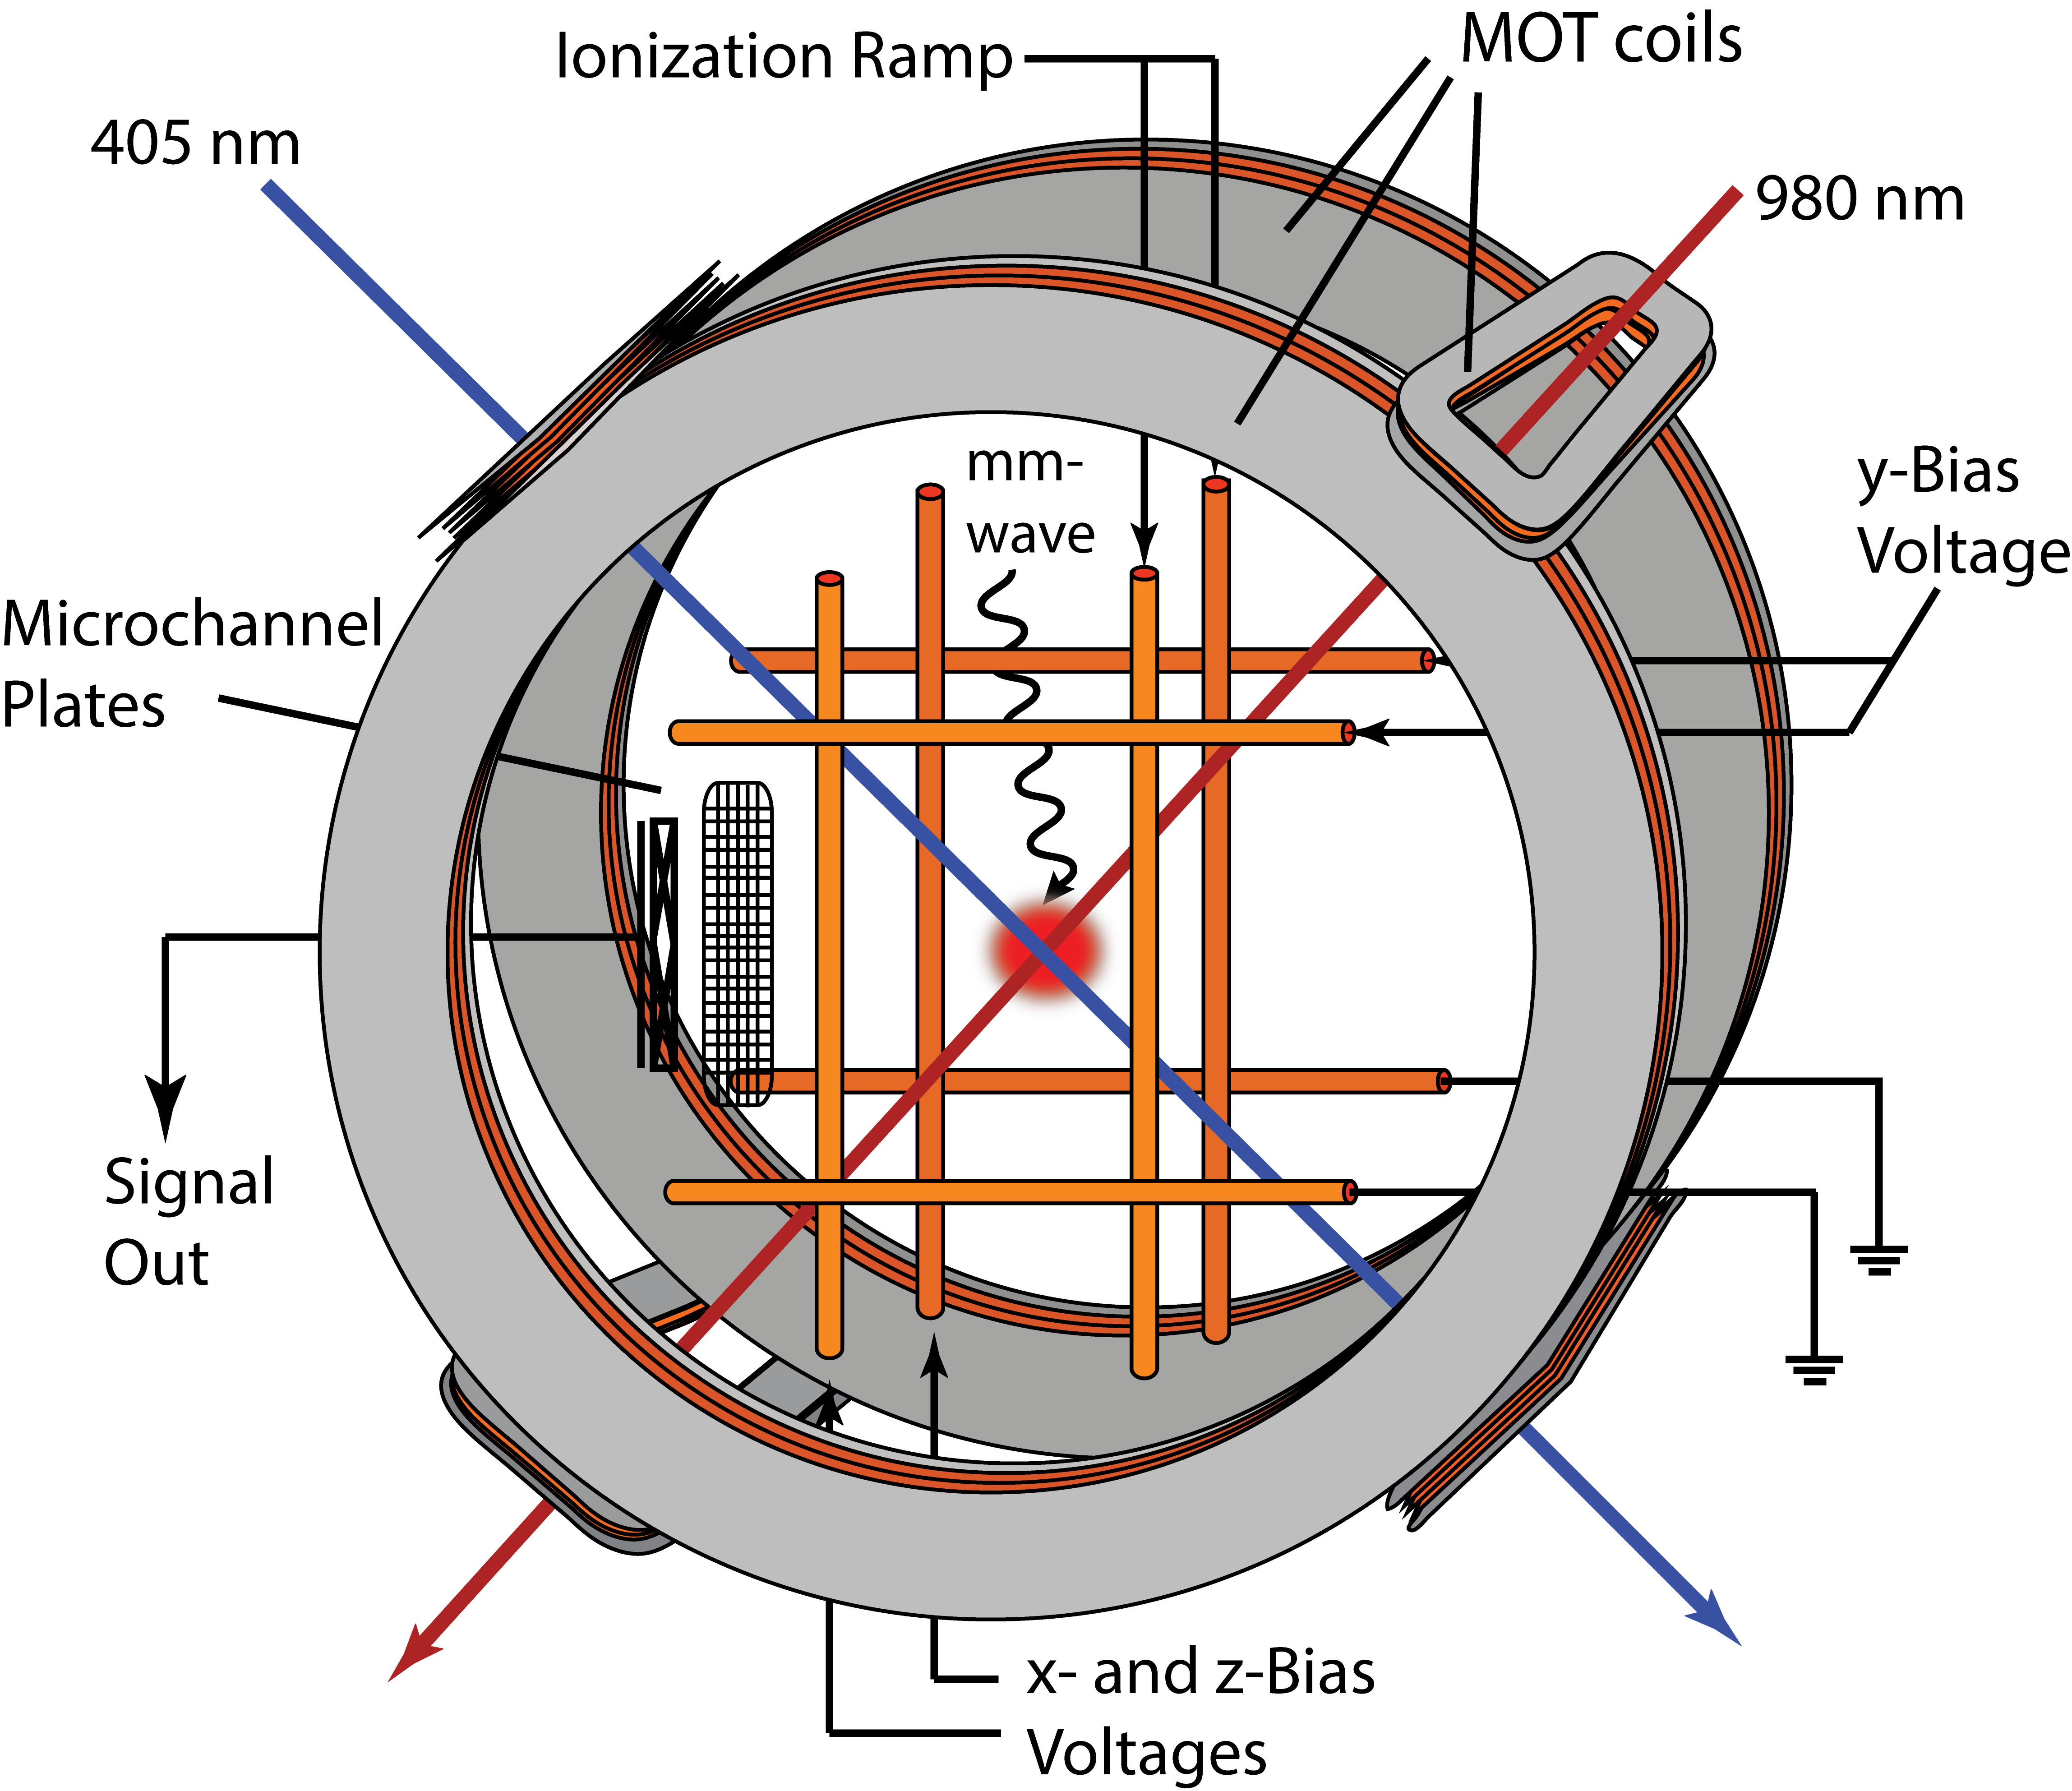
\includegraphics[scale = 1]{MOT.png}
\caption{\normalfont{Drawing of the apparatus, with the MOT cloud trapped in a magnetic field created by 2 MOT coils and cooled by a 770 nm laser (not shown). The rods provide a static field and an ionization field. A mm-wave from outside the vacuum chamber drives nd$_j$ $\rightarrow$ (n+1)d$_j$ transitions.}}
\label{MOT}
\end{center}
\end{figure}

\begin{figure}
\begin{center}
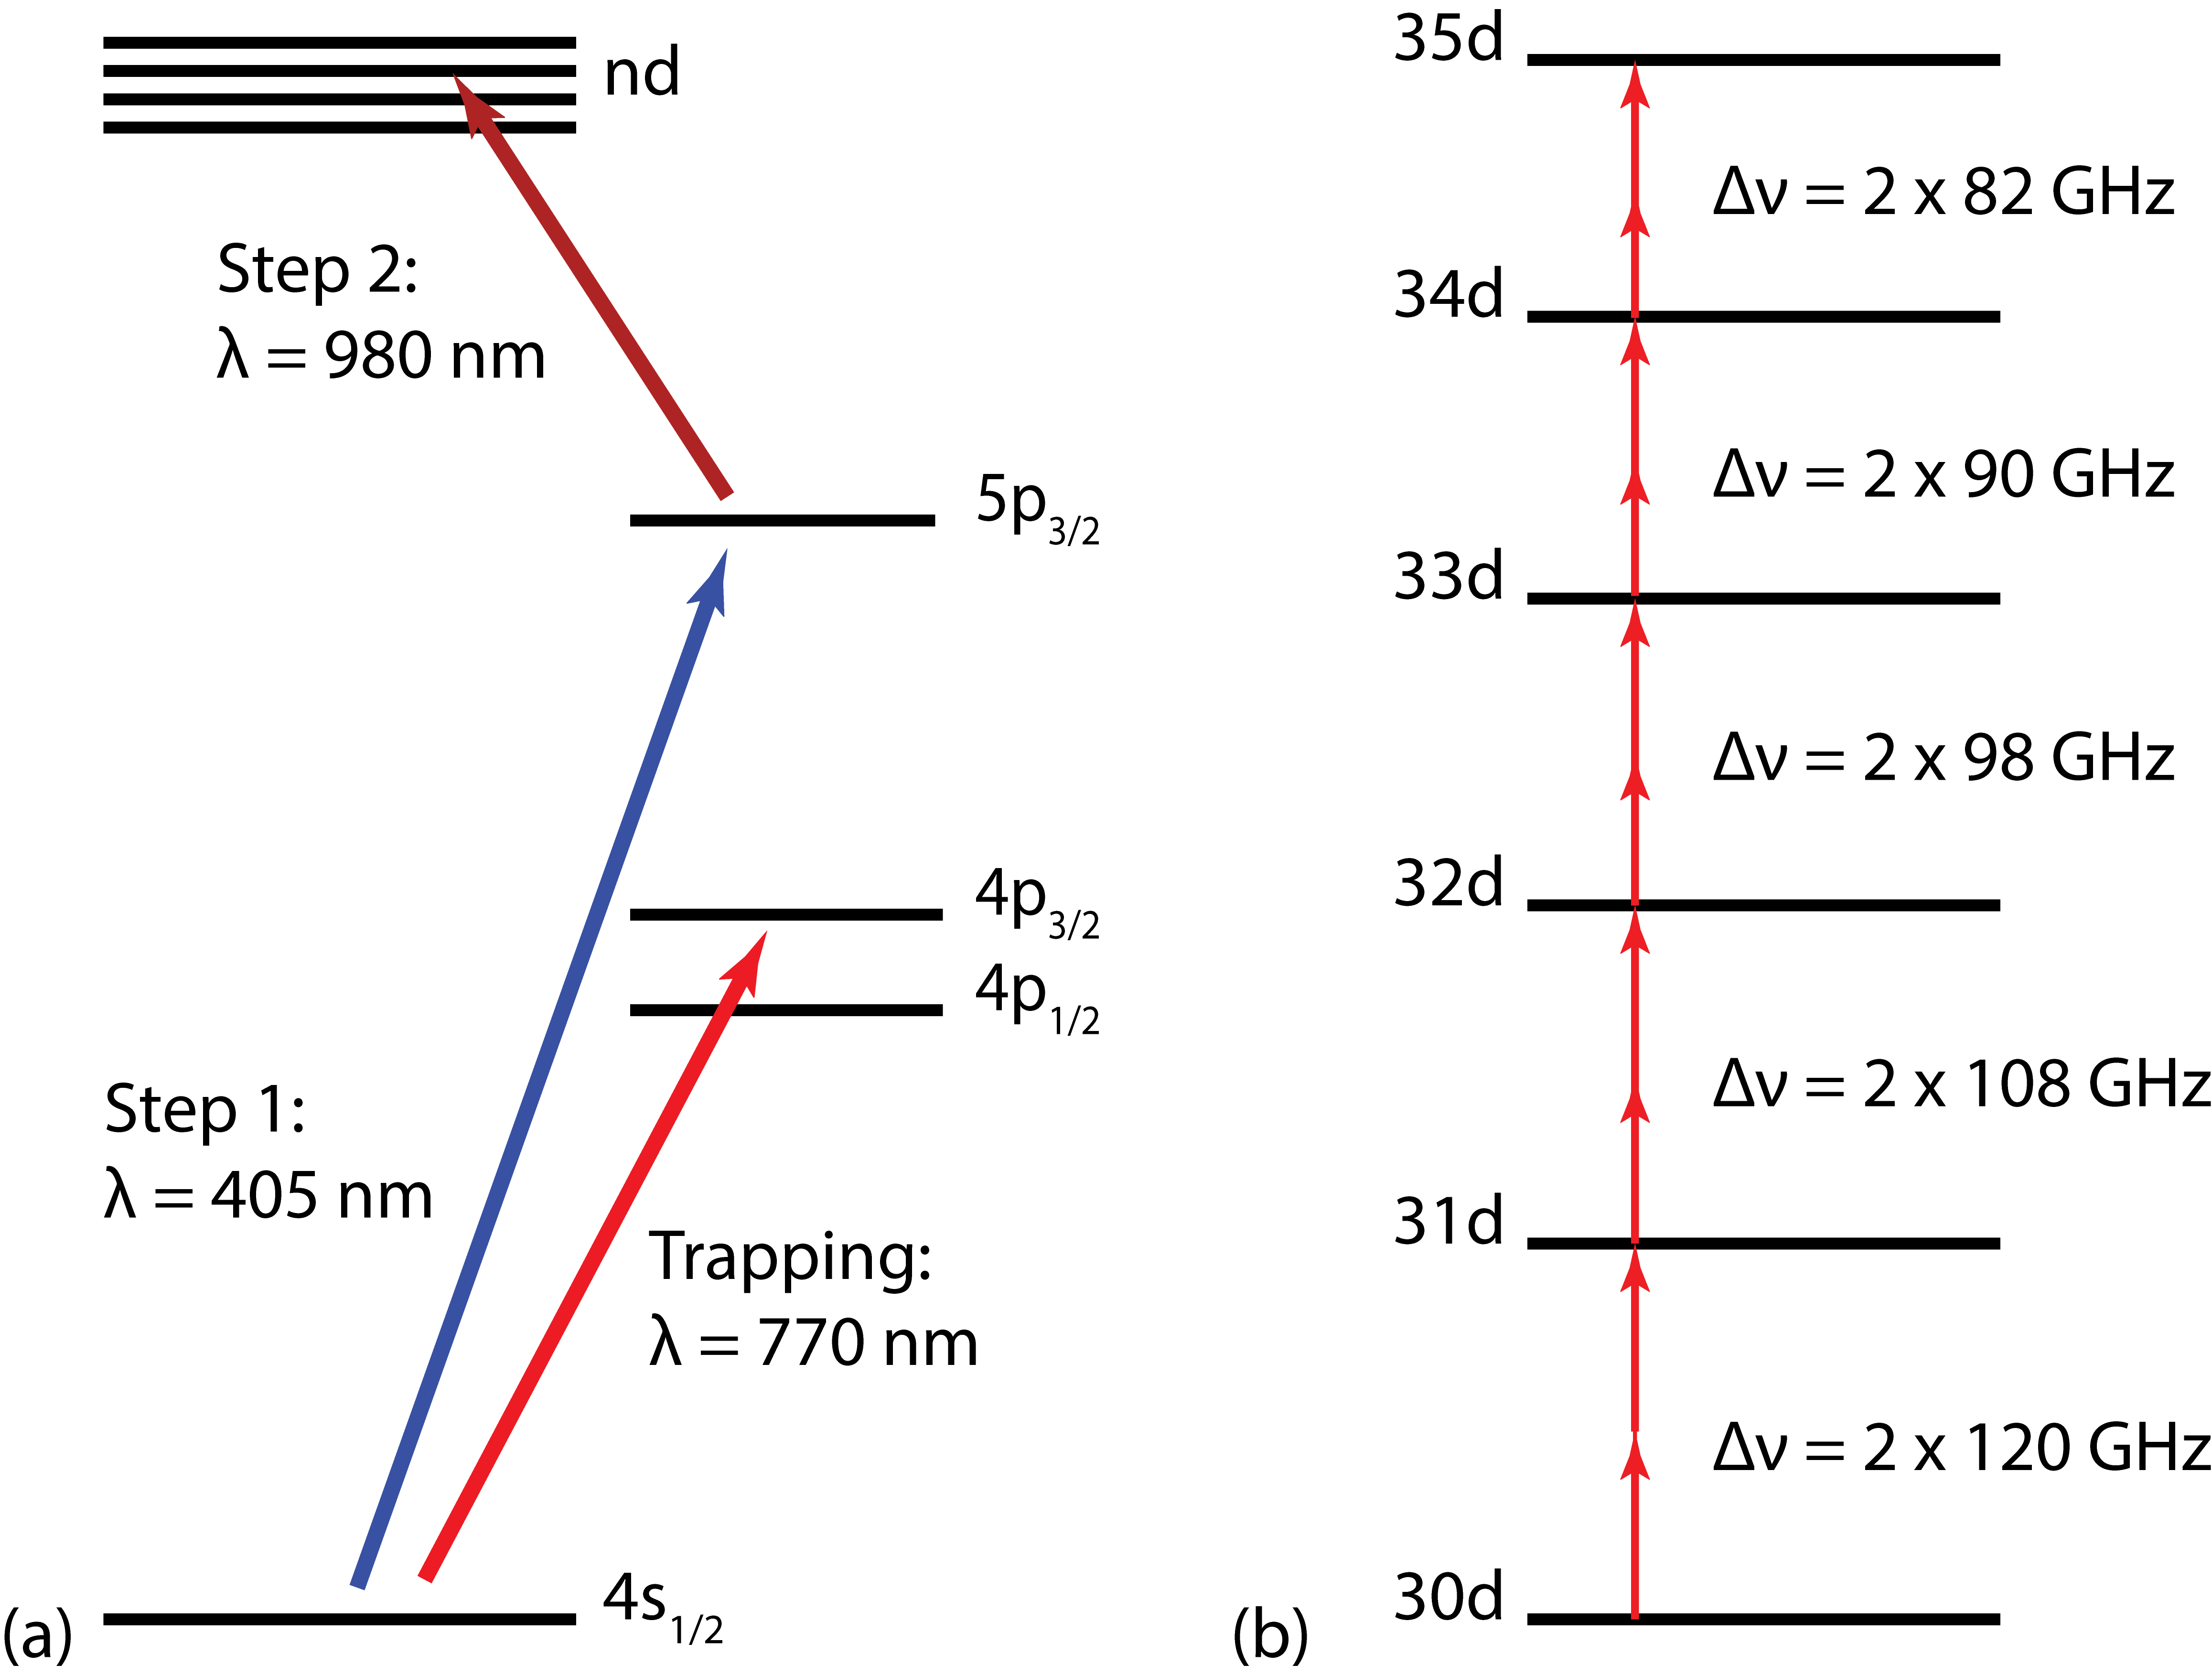
\includegraphics[scale = 1]{excitation.png}
\caption{\normalfont{(a) Rydberg excitation trapping \& (b) d-d excitation scheme}}
\label{Excitation}
\end{center}
\end{figure}
\section*{\large Static field elimination}
Energy levels of Rydberg states are sensitive to external static electric fields. Measured nd $\rightarrow$ (n+1)d transition frequencies vary quadratically with static field amplitude:
\begin{align*}
\boxed{\Delta \nu_{nd_j \rightarrow (n+1)d_j} = \nu_{0} - \frac{1}{2} \Delta \alpha E^2}
\end{align*}
%\begin{equation*}
%\resizebox{0.65\hsize}{!}{$\Delta \nu_{nd \rightarrow (n+1)d} = \nu_{0} - \frac{1}{2} \Delta \alpha E^2$},
%\end{equation*}
where $\Delta \alpha$ is the difference between the (n+1)d and nd polarizabilities, representing how strongly energy levels shift due to an external static electric field. 

\begin{figure}
\begin{center}
\includegraphics[scale = 0.8]{nulling.eps}
\includegraphics[scale = 0.8]{sumV.eps}
\includegraphics[scale = 0.8]{deltaV.eps}
\includegraphics[scale = 0.8]{Vy.eps}
\caption{\normalfont{ 33d\textsubscript{5/2}$\rightarrow$34d\textsubscript{5/2} DC Stark shifts \& field nulling}}
\label{nulling}
\end{center}
\end{figure}
%Static field elimination for 33d\textsubscript{5/2} $\rightarrow$ 34d\textsubscript{5/2} transition. 

Transition frequency is maximized when the static field components in all each of the orthogonal directions is zero. A DC bias in each direction nulls the field in that direction. 

\section*{\large Zero mm-wave power extrapolation}
While not a large effect, the energy shift caused by the mm-wave source is significant at our level of precision. This shift is directly proportional to the intensity of the interacting mm-wave. 

\begin{figure}
\begin{center}
\includegraphics[scale = 0.9]{33d52_PScans.eps}
\caption{\normalfont{Zero-power extrapolation for 33d\textsubscript{5/2} $\rightarrow$ 34d\textsubscript{5/2}}}
\label{Power}
\end{center}
\end{figure}

%Zero-power extrapolation for 33d\textsubscript{5/2} $\rightarrow$ 34d\textsubscript{5/2} transition after static field elimination. 
The y-intercept of the linear fit of the measured transition frequencies is the mm-wave-free transition frequency. The energy shifts from 0.35 to 0 relative intensity are on the order of a few kHz.\\

The 33d\textsubscript{5/2} $\rightarrow$ 34d\textsubscript{5/2} spacing can then be calculated:
\begin{align*}
\Delta \nu_0 = \textrm{2f\textsubscript{mm}} &= \textrm{179,496 MHz - 12.540 MHz} \\ &= \textrm{179,483.460(6) MHz}
\end{align*}



\section*{\large Ramsey's SOF, an alternative technique}
Ramsey's separated oscillatory field method removes the need for zero-power extrapolation. K atoms in the nd state are exposed to a double pulse of width $\tau$ and delay $T$ instead of a long, single pulse. 

\begin{figure}
\begin{center}
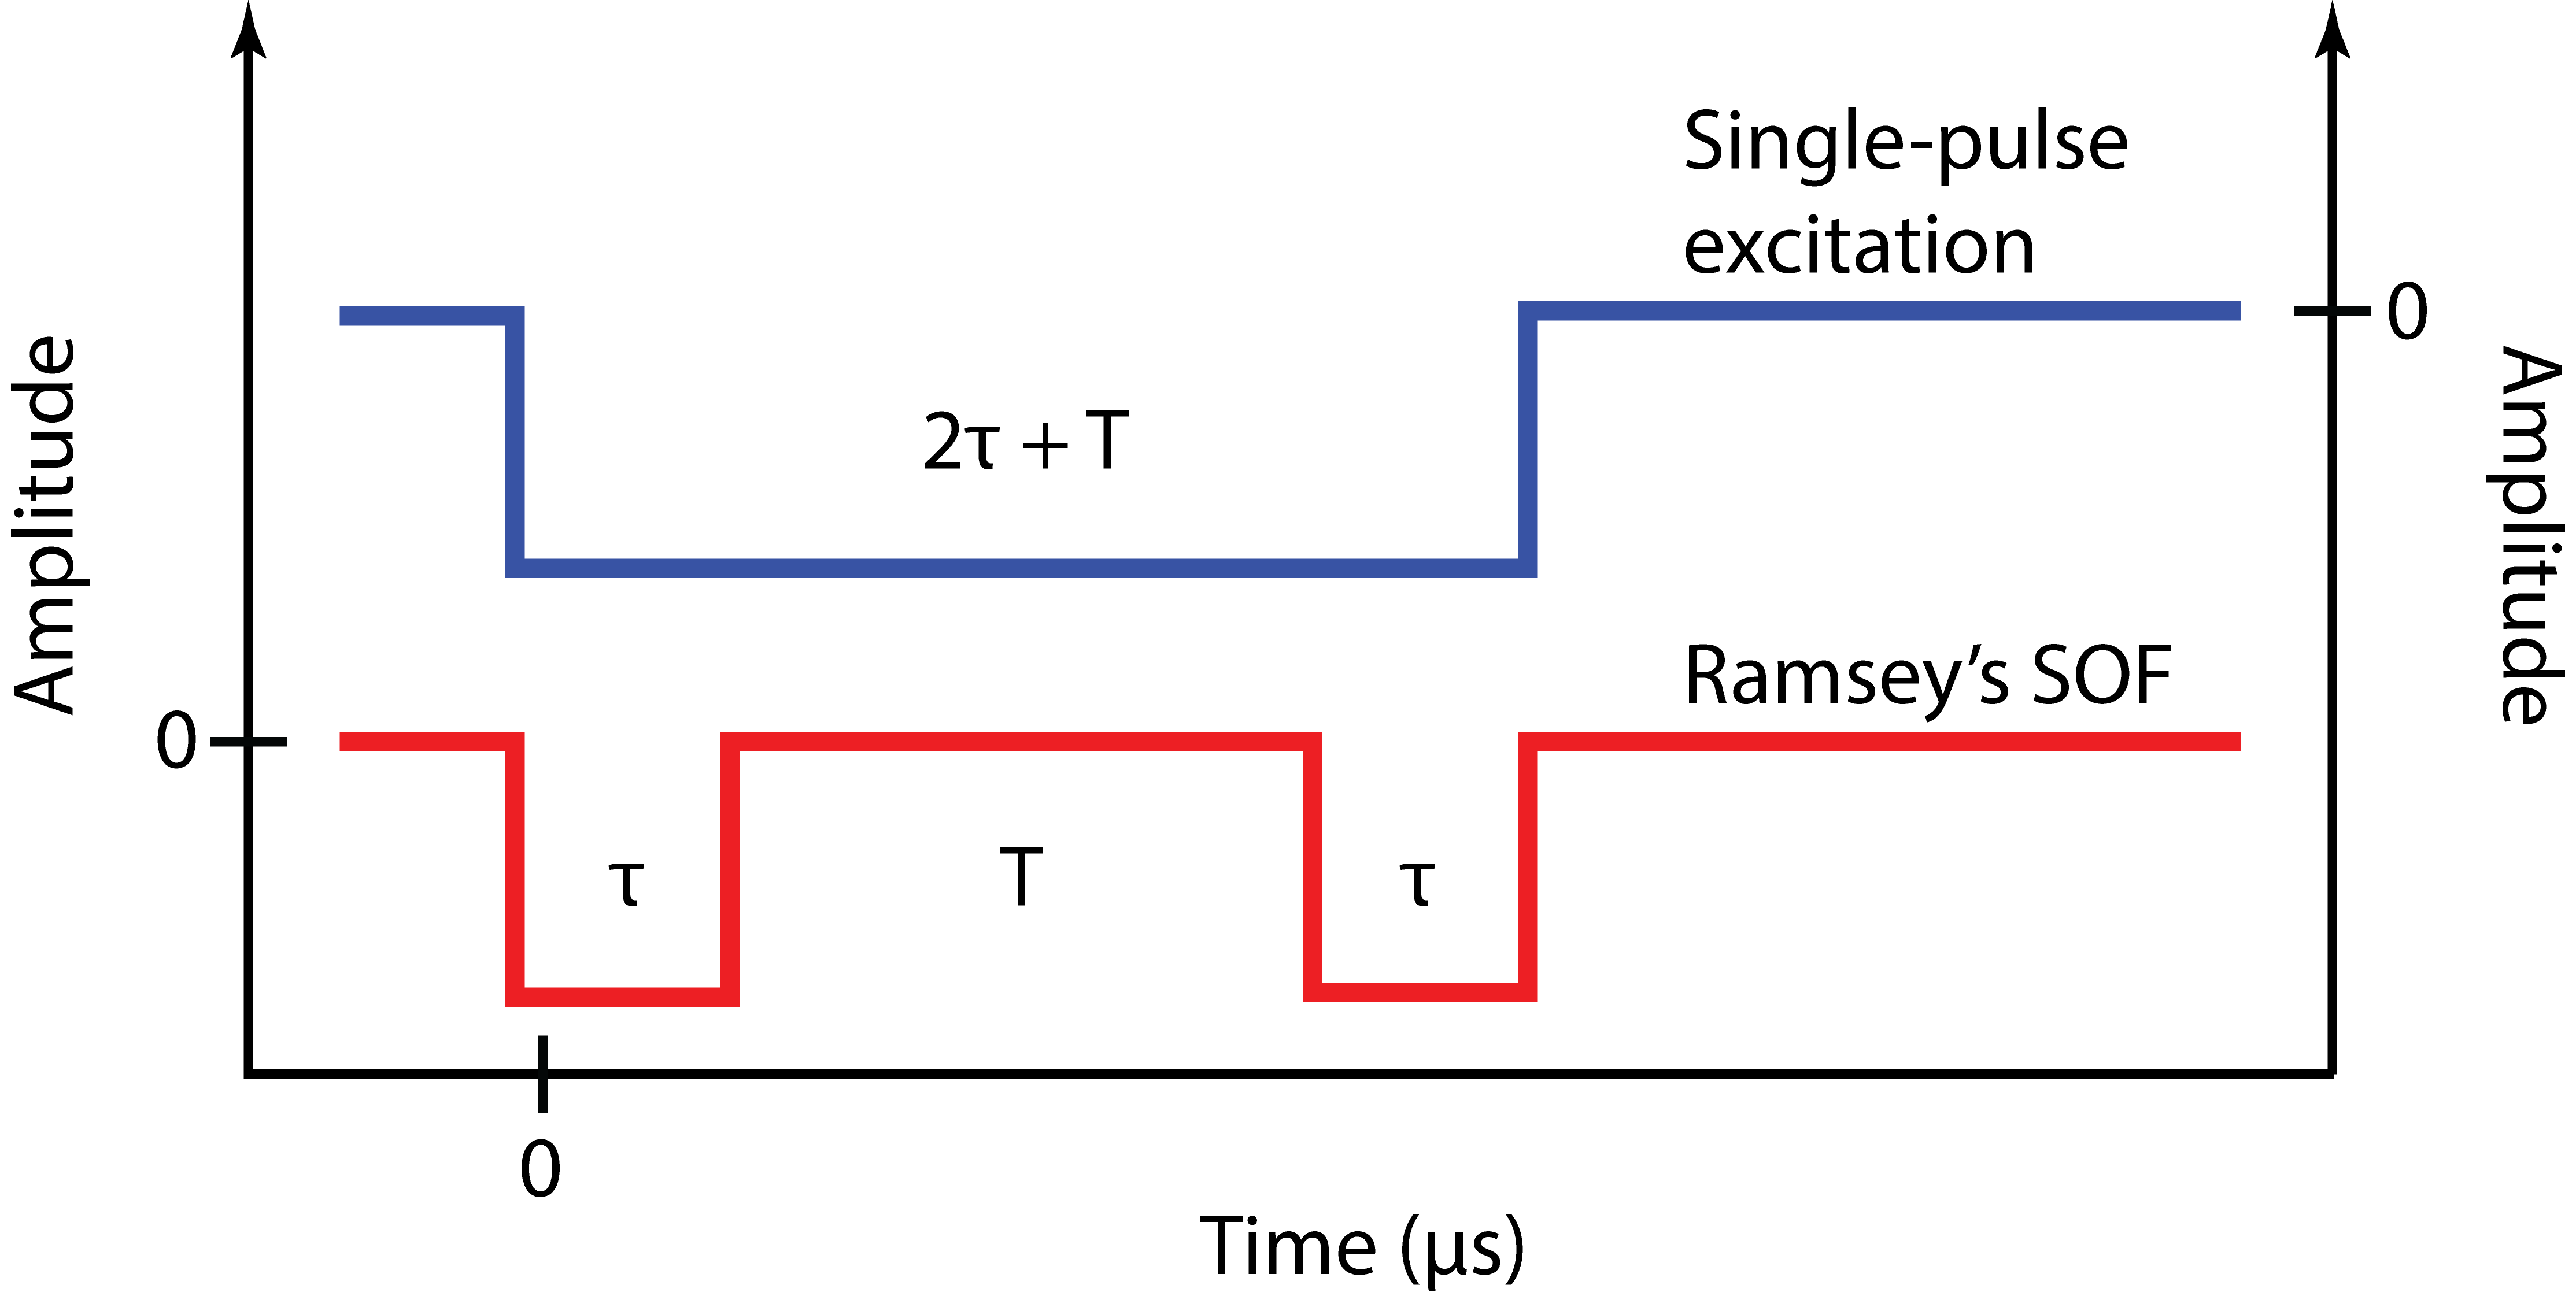
\includegraphics[scale=1]{Ramsey_excitation.png}
\caption{\normalfont{Single-pulse v. Ramsey's SOF scheme}}
\label{excitation scheme}
\end{center}
\end{figure}

A detuning scan reveals Ramsey fringes, as expected.

\begin{figure}
	\begin{center}
		\includegraphics[scale = 1]{fringes.eps}
		\caption{\normalfont{Ramsey fringes \& fit for 32d\textsubscript{5/2}$\rightarrow$33d\textsubscript{5/2}. Field-free spacing can be detected from the fit.} }
		\label{Ramsey fringes}
	\end{center}
\end{figure}
(n+1)d$_j$ state population oscillates as a function of $T$: 
\begin{align*}
\boxed{P_{(n+1)d_j} \propto {\cos}^{2}\left(\frac{\Delta_{0} T}{2}\right)}
\end{align*}
%\begin{equation*}
%\resizebox{0.45\hsize}{!}{$P_{(n+1)d} \propto {\cos}^{2}\left(\frac{\Delta_{0} T}{2}\right),$}
%\end{equation*}
where $\Delta_0=\omega_0-(E_{\text{(n+1)d}_j}-E_{\text{nd}_j})/\hbar$ is the beat frequency between the mm-wave and the atomic transition frequencies in zero oscillatory field. With known mm-wave frequency offset, fitting a cosine squared to a delay scan signal allows for determining the zero-power frequency for the 33d\textsubscript{5/2} $\rightarrow$ 34d\textsubscript{5/2} transition.

\begin{figure}
%\includegraphics[scale = 1]{data68.eps}
%\includegraphics[scale = 1]{data67.eps}
%\includegraphics[scale = 1]{data69.eps}
\includegraphics[scale = 1]{data68-67-69.eps}
\caption{\normalfont{Delay ($T$) scans at different $\omega_0$'s. Each corresponds to the same field-free interval 179,483.467(10) MHz}.}
\label{Ramsey}
\end{figure}

%The fit gives $\Delta_0/2\pi = \textrm{-0.4277 MHz}$. With an initial mm-wave frequency offset of $\textrm{-12.96 MHz}$, the field-free 33d\textsubscript{5/2} $\rightarrow$ 34d\textsubscript{5/2} spacing is:
%\begin{align*}
%\Delta \nu_0 &= \nu_{\textrm{offset}} - \Delta_0/2\pi + \textrm{179,496 MHz}\\
%&= \textrm{-12.96 MHz + 0.4277 MHz + 179,496 MHz} \\ 
%&= \textrm{179,483.47 MHz},
%\end{align*}
%consistent with the zero-power-extrapolated value to within a part in 10\textsuperscript{7}.

\section*{\large Determination of d-state quantum defects}
The absolute energies are given by:
\begin{align*}
\boxed{E_n = -\frac{hcR_K}{(n - \delta(n))^2}, \hspace{0.7cm} \delta(n) = \delta_0 + \frac{\delta_2}{(n-\delta_0)^2}}
\end{align*}
%\begin{equation*}
%\resizebox{0.45\hsize}{!}{$E_n = -\frac{hcR_K}{(n - \delta(n))^2},$}
%\end{equation*}
where $n$ is the principal quantum number, and $\delta(n)$ is parameterized by two coefficients, $\delta_0$ and $\delta_2$.
%\begin{equation*}
%\resizebox{0.5\hsize}{!}{$\delta(n) = \delta_0 + \frac{\delta_2}{(n-\delta_0)^2}.$}
%\end{equation*}


\begin{figure}
	\begin{center}
		\includegraphics[scale = 0.90]{d32_qd_new.eps}
		\includegraphics[scale = 0.90]{d52_qd_new.eps}
		\caption{\normalfont{nd$_j$ $\rightarrow$ (n+1)d$_j$ transition frequencies versus principal quantum number. A fit of the measured transition energies is be used to determine $\delta_0$ and $\delta_2$ for the d\textsubscript{3/2} and d\textsubscript{5/2} states. Residuals of the fit are less than 5$\times$10$^{\text{-8}}$ of the transition frequency.}}
		\label{qd}
	\end{center}
\end{figure}




\section*{\large Acknowledgments}
This research is supported by Colby College.

\end{multicols}

\end{document}
